\section{Background}
\label{sec:background}

\begin{figure}[t]
 \centering
 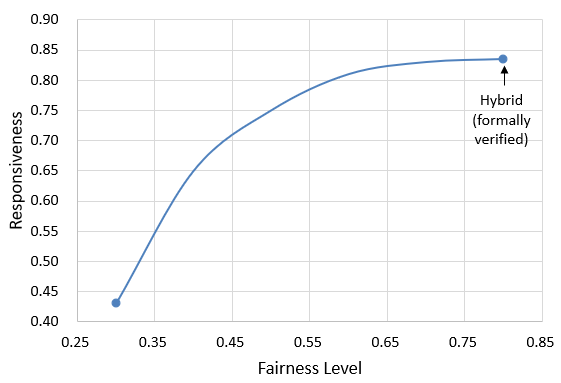
\includegraphics[width=0.82\linewidth]{./fig_tradeoff_curve.png}
 \caption{\textbf{Responsiveness--Fairness Trade-off Curve.} (grayscale-friendly). As responsiveness bias $\beta$ increases, fairness (Jain's index) decreases. BRS Hybrid reaches a balanced point, outperforming static policies.}
 \label{fig:trade-off}
\end{figure}

General-purpose operating systems balance throughput, fairness, and responsiveness---goals often in tension \cite{Bouron2018Battle,241774,1244943}. The trade-off is non-linear: as responsiveness bias rises, fairness can drop disproportionately, causing starvation and unpredictability \cite{10306992,4624248,67577}. As Figure~\ref{fig:trade-off} shows, increasing $\beta$ improves short-term latency but reduces fairness, motivating our hybrid design \cite{4624248,4663063}. Existing approaches to improve responsiveness fall into three categories: (1)~user-space prioritization and affinity tuning \cite{2020ThreadEK,1324648}, (2)~user-space schedulers atop kernel primitives \cite{7426385,917709}, and (3)~alternative kernel schedulers such as BFS or MuQSS \cite{10306992}. Each has drawbacks: user-space solutions lack deep control, and BFS/MuQSS compromise fairness or scalability \cite{Bouron2018Battle,8360522}.

Our investigation shows that modest kernel-level modifications can reshape this trade-off \cite{4663063,6365626}: small shifts in \textit{vruntime} calculation or runqueue choice yield significant latency drops for a negligible fairness sacrifice \cite{10306992,8360522}. BRS realizes this as a bounded responsiveness bias in the scheduler core, exposed through a controlled \texttt{/proc} surface for safe production deployment without application changes \cite{Bouron2018Battle,7426385,4624248}.

\textbf{Notation.} Fairness is the \emph{Jain's fairness index} $J = \frac{(\sum_{i=1}^n x_i)^2}{n \sum_{i=1}^n x_i^2}$ \cite{Guo2013JainFairness}; tail latency is $L_{95}$ (95\textsuperscript{th} percentile). $\mathbb{E}[\cdot]$ is expectation, $\mathbf{1}\{\cdot\}$ an indicator. Parameters $(\alpha,\beta)$ control responsiveness bias; $\kappa$ is the adaptation gain.
